\frame{\titlepage}


\begin{frame}{Abstract}
I will demonstrate the solution with all its steps (and missteps) to the boundary layer problem
\begin{equation}
    \varepsilon y'' = y\cdot y' - y, \label{eq:diff_eq}
\end{equation}
such that
\begin{equation}
    y(0) = 1 \qq{and} y(1) = -1 \qq{and where} \varepsilon \ll 1. \label{eq:boundary_conditions}
\end{equation}
  The journey towards the solution will take us on an excurse through some basics of \emph{perturbation theory} and \emph{asymptotic approximation matching}. I will demonstrate visualizations that will give you insight into the reasoning behind the steps taken towards the solution serving as an exhibition for the leverage in problem solving accessible to us through the computational power at our fingertips.
\end{frame}

\begin{frame}{Outline}
    \tableofcontents[subsectionstyle=hide, subsubsectionstyle=hide]
\end{frame}

\section{Motivation}%
\label{sec:motivation}

\begin{frame}{Classifying the problem}
    \begin{equation*}
\varepsilon \textcolor<2,3,4,6>{Orange}{y}\textcolor<4,6>{Orange}{''}\only<6>{\textcolor{Orange}{(x)}}
        = \textcolor<2,3,5,6,7>{Orange}{y}\only<6>{\textcolor{Orange}{(x)}}\textcolor<7>{Orange}{\cdot}\textcolor<2,3,6,7>{Orange}{y}\textcolor<6,7>{Orange}{'}\only<6>{\textcolor{Orange}{(x)}}
        - \textcolor<2,3,5,6>{Orange}{y}\only<6>{\textcolor{Orange}{(x)}}
    \end{equation*}
   such that
   \begin{equation*}
       \textcolor<8>{Orange}{y(0) = 1} \qq{and} \textcolor<8>{Orange}{y(1) = -1} \qq{and where} \varepsilon \ll 1.
   \end{equation*}
   \begin{description}
       \item<2->[\emph{ordinary}] single unknown function \only<3>{\textcolor{gray}{(as opposed to a PDE)}}
       \item<4->[\emph{second-order}] contains a second order derivative
       \item<5->[\emph{first-degree}] highest degree of the unknown function is \(1\)
       \item<6->[\emph{homogeneous}] does not contain a free term in the \(x\) variable
       \item<7->[\emph{non-linear}] contains a mixed term
       \item<8->[\emph{(boundary-value)}] constrained by values on the boundaries
   \end{description}
\end{frame}

\begin{frame}{Similar Differential Equations}
    \only<1,2>{What is the biggest problem in solving this DE? \\} \pause
    \alt<2>{It is \emph{non-linear} !}{Have we encountered other non-linear DEs?}
    \pause\pause
    \begin{itemize}
        \item Newtons gravitational equation
        \pause \textcolor{gray}{(ordinary, second-order, second-degree, homogeneous, non-linear)} 
        \pause
        \item Simple pendulum
        \pause \textcolor{gray}{(ordinary, second-order, homogeneous, non-linear)} 
    \end{itemize}
    \pause How did we manage to solve these equations?
\end{frame}

\begin{frame}
        \begin{figure}[h!]
            \centering
            \temporal<2>{\includepdftex{comparison_of_numerical_solution_to_small_angles_pendulum_time_span_0.0_1.6.pdf_tex}}{\includepdftex{comparison_of_numerical_solution_to_small_angles_pendulum_time_span_0.0_6.3.pdf_tex}}{\includepdftex{comparison_of_numerical_solution_to_small_angles_pendulum_time_span_0.0_19.0.pdf_tex}}
            \caption{Comparison of the numerical solution and the small angle approximation of the simple pendulum DE for the initial angle
                \(\varphi(0) = \pi/4 \) and \(\dot{\varphi}(0) = 0\).}
            \only<3>{}
        \end{figure}
\end{frame}

\begin{frame}{Classifying the problem}
    \begin{equation*}
        \varepsilon y'' = y\cdot y' - y
    \end{equation*}
   such that
   \begin{equation*}
       y(0) = 1 \qq{and} y(1) = -1 \qq{and where} \textcolor<2>{Orange}{\varepsilon \ll 1}.
   \end{equation*}
   \begin{description}
       \item[\emph{ordinary}] single unknown function
       \item[\emph{second-order}] contains a second order derivative
       \item[\emph{first-degree}] highest degree of the unknown function is \(1\)
       \item[\emph{homogeneous}] does not contain a free term in the \(x\) variable
       \item[\emph{non-linear}] contains a mixed term
       \item[\emph{(boundary-value)}] constrained by values on the boundaries
       \item<2>[\emph{singularly-perturbed}] contains one small term
   \end{description}
\end{frame}

\subsection{Numerical Methods}%
\label{sub:numerical_methods}

\begin{frame}
    \only<1>{How good is our numerical solution?}
    \only<2>{\begin{remark}[Analytical solution - \cite{salas2014}]
        There is an analytical solution to the pendulum DE in the form 
        \begin{gather*}
            \varphi(t) =  2 \cdot \arcsin(\sin(\varphi_0 / 2) \cdot \operatorname{cd}(t \cdot \sqrt{g / L},\, 
            \sin^2(\varphi_0 / 2))),\text{ where} \\
            \begin{gathered}
                \operatorname{cd}(u, m) = \operatorname{cn}(u, m) / \operatorname{dn}(u, m) \\
                \operatorname{cn}(u, m) = \cos(\operatorname{am}(u,m)) \quad \operatorname{dn}(u, m) = \dv{u} (\operatorname{am}(u,m))
            \end{gathered}
        \end{gather*}
        and \(\operatorname{am}(u, m) = \varphi\) is the \emph{Jacobi amplitude} which is the upper-bound of the integral such
        that \[
            u = \int_0^\varphi \frac{\dd \vartheta}{\sqrt{1 - m \sin^2(\vartheta)}}.
        \] 
\end{remark}}
\end{frame}

\begin{frame}
    \begin{figure}[h!]
        \centering
        \includepdftex{comparison_of_analytical_solution_to_numerical_solution_time_span_0.0_19.0.pdf_tex}
        \caption{Comparison of the analytical solution and the numerical solution of the simple pendulum DE for
        the initial angle \(\varphi(0) = \pi/4 \) and \(\dot{\varphi}(0) = 0\).}
    \end{figure}
\end{frame}

\begin{frame}
    Why would we want to bother with perturbation methods\alt<1>{?}{, when we can make the numerical solution arbitrarily more
    precise?} \pause \pause
    \begin{itemize}
        \item<+-> Perturbation methods approximation is interpretable
        \item<+-> We can prove some good qualities about the solution \pause \textcolor{gray}{(uniform convergence, etc.)} \pause
        \item<+-> Numerical solution is not guaranteed to be correct
        \item<+-> \emph{Size of the latent space for the solution!} \pause \textcolor{gray}{\emph{(we cannot search the whole space and find
            all the solutions numerically)}}
    \end{itemize}
\end{frame}

\note{
    \begin{description}
        \item[\emph{Interpretability:}] increasing/decreasing, number of roots, etc.
        \item[\emph{Numerical stability:}] some good qualities are guaranteed
            \begin{enumerate}
                \item when the respective derivatives are
            "well-behaved" (respective means the ones used by the method)
                \item when we have some guarantees for the stability of the solutions (Lyapunov stability)
            \end{enumerate}
        \item[\emph{Latent-space size:}]\leavevmode
            \begin{enumerate}
                \item we only have an \emph{ODE}. The problem is magnified when we have a \emph{PDE}! (same reason why
                    we cannot interpret solutions of NN well)
                \item How do we make the numerical solutions and what would be the problem? \emph{Latent-space stability} 
            \end{enumerate}
        \item[\emph{Numerical solution:}] perturbation methods to make a better (more efficient) numerical solution - This will be our case...
    \end{description}
}


\begin{frame}
    \only<1>{How precise is a perturbation solution?}
    \only<2>{
        \begin{remark}[Perturbation solution - \cite{belendez2006}]
            There is an approximation to the simple pendulum problem based on a homotopy perturbation method. It is
            uniformly convergent and is precise from the first few terms of the expansion.
        \end{remark}
    }
\end{frame}

\begin{frame}
    \begin{figure}[h!]
        \centering
        \includepdftex{comparison_of_analytical_solution_to_perturbation_methods_solution_time_span_0.0_19.0.pdf_tex}
        \caption{Comparison of the perturbation solution and the analytical solution of the simple pendulum DE for
        the initial angle \(\varphi(0) = \pi/4 \) and \(\dot{\varphi}(0) = 0\).}
    \end{figure}
\end{frame}

\section{Theory}%
\label{sec:theory}

\subsection{Mathematical Basics}%
\label{sub:mathematical_basics}

\begin{frame}
   \begin{theorem}[Taylor's theorem]
       Given a function \(f(\varepsilon)\), suppose its \((n+1)\)st derivative \(f^{(n+1)}\) is continuous for
       \(\varepsilon_a < \varepsilon < \varepsilon_b\). Suppose that the points \(\varepsilon,\varepsilon_0 \in (\varepsilon_a,
       \varepsilon_b)\). Then
       \[
           f(\varepsilon) = f(\varepsilon_0) + (\varepsilon - \varepsilon_0)f'(\varepsilon_0) + \ldots
           + \frac{1}{n!}(\varepsilon - \varepsilon_0)^n f^{(n)}(\varepsilon_0) + R_{n+1},
       \]
       where the error term \(R_{n+1}\) is given by
       \[
           R_{n+1} = \frac{1}{(n+1)!}(\varepsilon - \varepsilon_0)^{n+1} f^{(n+1)}(\xi),
       \]
       and \(\xi \in ]\varepsilon, \varepsilon_0 [\)
    \end{theorem}
\end{frame}

\begin{frame}
    \begin{definition}[Bachmann-Landau Symbols - \cite{holmes2012}]\leavevmode
        \begin{enumerate}
            \item<+-> \(f = O(\varphi)\) as \(\varepsilon \to \varepsilon_0^{+}\) if there is a constant \(k\) and
                \(\tilde{\varepsilon}\) so that \[
                    \left| f(\varepsilon) \right| \le k \left| \varphi(\varepsilon) \right| \qq{for} \varepsilon_0
                    < \varepsilon < \tilde{\varepsilon}
                \] 

            \item<+-> \(f = o(\varphi)\) as \(\varepsilon \to \varepsilon_0^{+}\) if \(\forall \delta > 0\) there is
                a \(\tilde{\varepsilon}\) so that \[
                    \left| f(\varepsilon) \right| \le \delta \left| \varphi(\varepsilon) \right| \qq{for} \varepsilon_0
                    < \varepsilon < \tilde{\varepsilon}
                \] 
        \end{enumerate}
    \end{definition}
\end{frame}

\note[itemize]{
    \item What does our \(\varepsilon \ll 1\)  mean in terms of the Bachmann-Landau symbol
}

\subsection{Perturbation Theory}%
\label{sub:perturbation_theory}

\note[itemize]{
    \item Long history of the Perturbation Theory (Legendre, Poincaré, Laplace)
}

\begin{frame}
    \begin{definition}[Asymptotic approximation - \cite{holmes2012}]
        Given a function \(f(\varepsilon)\) and \(\varphi(\varepsilon)\) we say that \(\varphi(\varepsilon)\) is an
        \emph{asymptotic approximation} to \(f(\varepsilon)\) as \(\varepsilon \to \varepsilon_0^{+}\) whenever \(f
        = \varphi + o(\varphi)\) as \(\varepsilon \to \varepsilon_0^{+}\). We write \(f \sim \varphi\) as \(\varepsilon
        \to \varepsilon_0^{+}\).
    \end{definition}
\end{frame}

\begin{frame}
    \begin{definition}[Asymptotic expansion - \cite{holmes2012}]
        \begin{enumerate}
            \item The sequence of functions \(\varphi_1(\varepsilon), \varphi_2(\varepsilon),\ldots\) form an
              \emph{asymptotic sequence} (are \emph{well ordered}) as \(\varepsilon \to \varepsilon_0^{+}\) if
              \(\varphi_{m+1} = o(\varphi_m)\) as \(\varepsilon \to \varepsilon_0^{+}\) for \(\forall m\).
                \pause \(\varphi_m\) are called the \emph{basis functions}. \pause
            \item<+-> Let \(\varphi_1(\varepsilon), \varphi_2(\varepsilon),\ldots\) be basis functions. Then
                \(f(\varepsilon)\) has an \emph{asymptotic expansion} to \(n\) terms for this sequence if \[
                    f =\sum_{k = 1}^{m} a_k \varphi_k + o(\varphi_m) \qq{for} m \in \hat{n} \qq{as} \varepsilon \to
                    \varepsilon_0^{+},
                \] 
                where \(a_k\) are independent of \(\varepsilon\). We can write \[
                    f \sim a_1 \varphi_1(\varepsilon) + a_2 \varphi_2(\varepsilon) + \ldots + a_n \varphi_n(\varepsilon)
                    \qq{as} \varepsilon \to \varepsilon_0^{+}.
                \]
        \end{enumerate}
    \end{definition}
\end{frame}

\begin{frame}{Asymptotic Solution of the Projectile Problem}
    \[
        \textcolor<1,2,3>{Orange}{\dv[2]{x}{t} = - \frac{g \cdot R^2}{(x + R)^2}} \qq{for} \textcolor<1,2,3>{Orange}{0 < t}.
    \]  \pause First we scale the equation to make the approximation easier \pause
    \begin{align*}
        \tau &= t \cdot g / v_0 \\
        y(\tau) &= x(t) \cdot g / v_0^2
    \end{align*} \pause Doing so transforms the problem into 
    \[
        \textcolor<4->{Orange}{\dv[2]{y}{\tau} = - \frac{1}{(1 + \varepsilon y)^2}} \qq{for} \textcolor<4->{Orange}{0 < \tau},
    \] where \[
        \textcolor<4->{Orange}{y(0) = 0} \qq{and} \textcolor<4->{Orange}{y'(0) = 1} \qq{and} \textcolor<4->{Orange}{\varepsilon = v_0^2 / Rg}.
    \] 
\end{frame}

\begin{frame}
    \begin{figure}[h!]
      \centering
      \includepdftex{comparison_of_numerical_perturbation_and_linearized_projectile_problem.pdf_tex}
      \caption{Comparison of the two term approximation, the linearised problem (one-term approximation) and the
      numerical solution for \(\varepsilon = 1/10\)} 
    \end{figure}
\end{frame}

\subsection{Boundary Layers}%
\label{sub:boundary_layers}
\begin{frame}{Boundary Layer}
  A boundary layer in lay terms is an interval of the solution of a DE where the derivative is large compared with
  surrounding times.
\end{frame}

\begin{frame}
  \begin{figure}
    \centering
    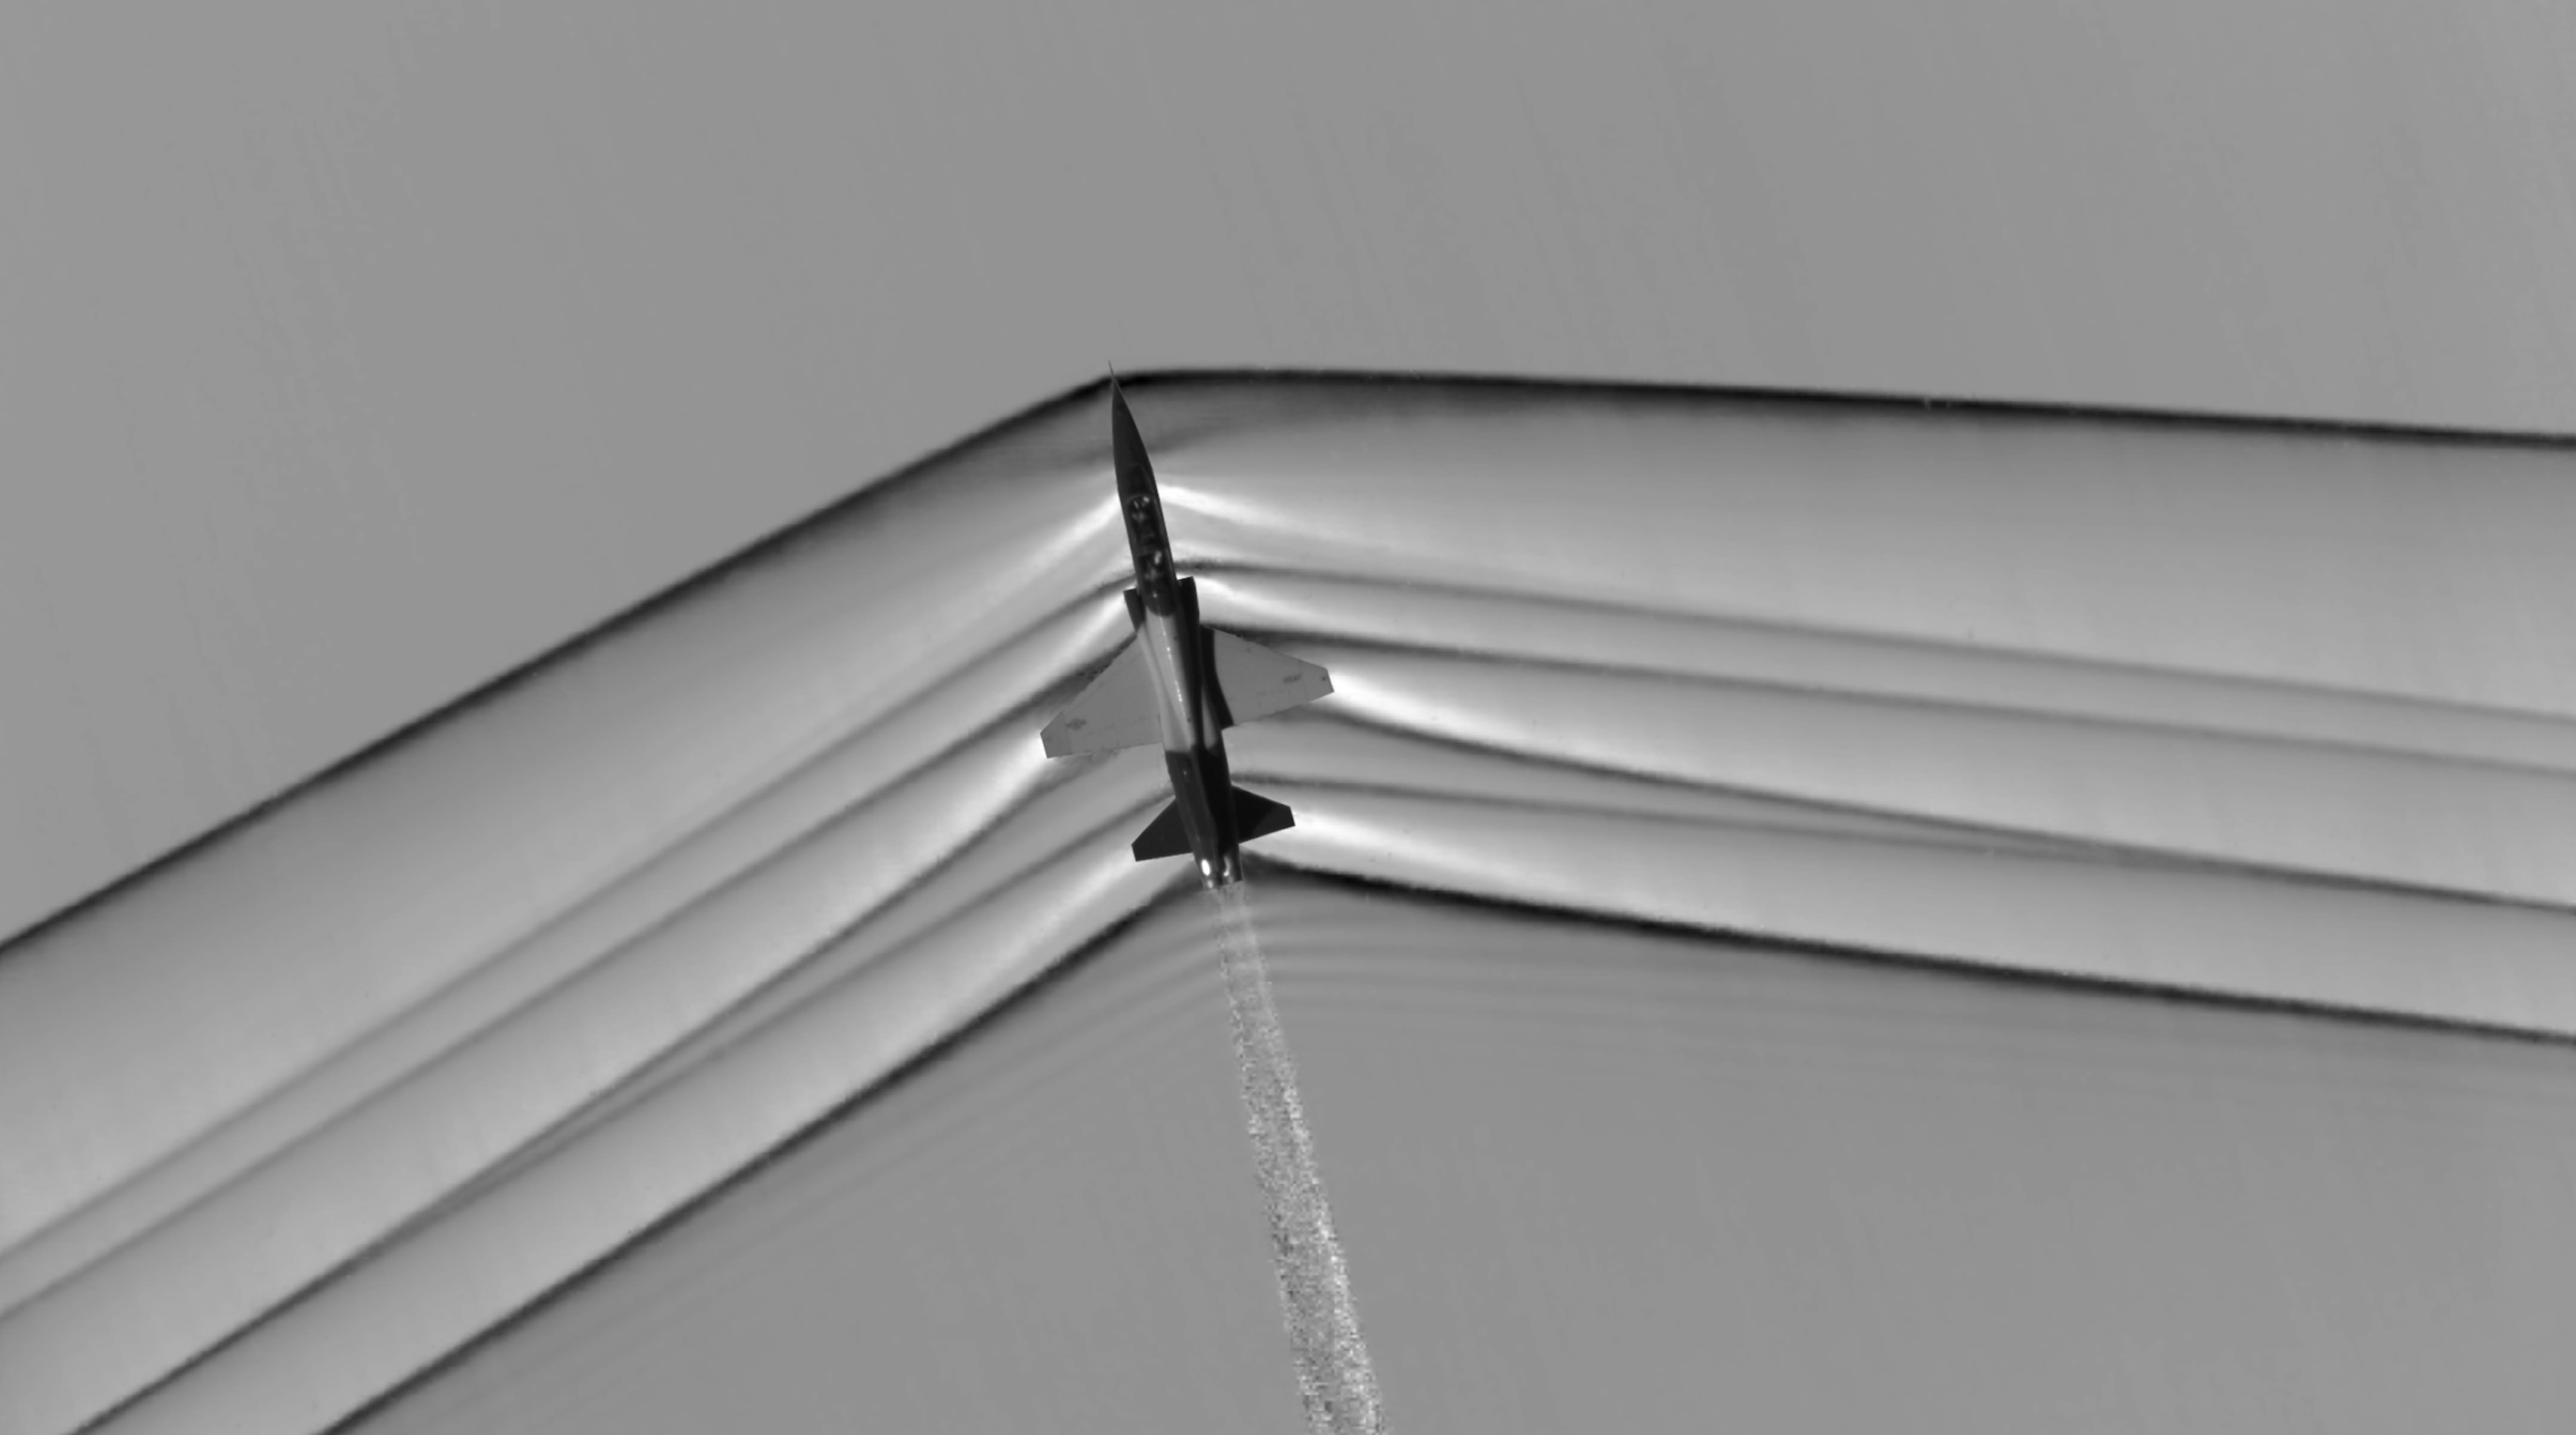
\includegraphics[width=0.8\textwidth]{Supersonic_airflow_Shlieren.jpg}
    \caption{Shlieren image of the air waves of a supersonic airflow produced by a fighter jet \emph{[Source: NASA (2015)]}}
  \end{figure}
\end{frame}


\note[itemize]{
    \item Why we cannot use a numerical solution blindly? (We would not find the initial condition of the shooting because the solutions \emph{B0} and \emph{B1} are too chaotic with dependence on \(\varepsilon\))
}

\section{Solution of the DE}%
\label{sec:solution_of_the_de}


\subsection{Locating the Boundary Layers}%
\label{sub:locating_the_boundary_layers}

\begin{frame}{Plausibility Argument of no Border Boundary Layers - \cite{holmes2012}}
    If we are looking for a boundary layer at \(x = 0\), then \(y' < 0\) and if we assume that \(y'' > 0\), then
    \(\varepsilon y'' > 0\), but \(y\cdot (y' - 1)\) on the left hand side is both \(>0\) on some interval and \(<0\).
    Therefore we can rule out any boundary layers at the interval borders for \(y'' > 0\).
\end{frame}


\subsection{Symmetry of the Unknown}%
\label{sub:symmetry_of_the_unknown}
\begin{frame}
  Is there any symmetry in the DE? \\ \pause
  \[
      (x,y) \to (1-x, -y)
  \] 
\end{frame}

\subsection{Phase Portrait}%
\label{sub:phase_portrait}

\begin{frame}{Phase Portrait of the DE}
    \alt<1>{
        \begin{equation*}
            \varepsilon y'' = y\cdot y' - y
        \end{equation*}
    }{
        \begin{align*}
            y'(t) &= z(t) \\
            z'(t) &= \frac{1}{\varepsilon} \cdot y(t) \cdot (z(t)-1)
        \end{align*}
    }\pause
\end{frame}

\begin{frame}
  \begin{figure}
    \centering
    \includepdftex{phase_portrait_arrows.pdf_tex}
    \caption{Arrows representing the vector field of our system of differential equations}
  \end{figure}
\end{frame}

\begin{frame}
    \alt<1>{
        \begin{figure}[h!]
            \centering
            \includepdftex{phase_portrait_imaginary_particle_trace_no_initial_vlines.pdf_tex}
            \caption{Trajectories of imaginary particles in the phase portrait of our system of differential equations
            for \(\varepsilon = 0.1\)}
        \end{figure}
    }{
        \begin{figure}[h!]
            \centering
            \includepdftex{phase_portrait_imaginary_particle_trace_initial_vlines.pdf_tex}
            \caption{Trajectories of imaginary particles in the phase portrait of our system of differential equations
                for \(\varepsilon = 1\) with the boundary condition hyperplanes}
        \end{figure}
    }
    \pause
\end{frame}

\begin{frame}
  \begin{figure}
    \centering
    \includepdftex{phase_portrait_solutions_B0_M_B1.pdf_tex}
    \caption{Solutions \(B_0\), \(M\) and \(B_1\) in the phase plane of the DE}
  \end{figure}
\end{frame}

\note[itemize]{
    \item Conservativeness of the system (trajectories do not overlap)
}

\subsection{Perturbation Theory}%
\label{sub:perturbation_theory}

\subsubsection{Outer Solution}%
\label{ssub:outer_solution}
\begin{frame}{Outer Solution}
  \pause \[
      y_0(x) = x + a \qq{for some} a \in \R
  \] \pause \[
    y_0^{L}(x) = 1 + x \qq{and} y_0^{R}(x) = x - 2
  \] 
\end{frame}

\subsection{Inner Solution}%
\label{sub:inner_solution}
\begin{frame}{Scaling}
    For the boundaries, we have to scale the solutions as 
    \[
        X \equiv \frac{x - x_0}{\delta},
    \] where \(\delta\) is the thickness of the layer and \(\delta = \delta(\varepsilon)\).
    \pause
    \[
        Y(X) \equiv y(x) = y(x_0 + \delta X)
    \] 
    \pause If \(\delta\) is chosen correctly, then \(Y\) and all its derivatives should be \(O(1)\) as \(\varepsilon \to
    0^{+}\) and we can find the limit when \(\varepsilon / \delta^2 = 1 / \delta\) or \(\delta = \varepsilon\). \pause
    The inner equation layer is \[
        \dv[2]{Y}{X} = Y \dv{Y}{X} - \varepsilon Y.
    \] 
\end{frame}

\begin{frame}{Inner Solutions}
    Solving the equation using the same expansion get us \[
        Y_0(X) = b \cdot \operatorname{tanh}(c - \frac{b}{2}\cdot X)
    \] \pause Composing the solutions \[
        \tilde{y} = y_\text{outer} + Y_\text{inner} - y_\text{match}
    \] \pause
    When we create these composite solutions, we get
        \begin{align*}
            \tilde{y}^{M} &= x - \frac{1}{2} - \frac{3}{2} \cdot \operatorname{tanh}\left[ \frac{3}{4\varepsilon} (x
            - \frac{1}{2}) \right]  + O(\varepsilon)\\
            \tilde{y}^{B0} &= x - 2 \cdot \operatorname{tanh}\left[ \frac{x}{\varepsilon}
            - \operatorname{tanh}^{-1}(1/2) \right] + O(\varepsilon) \\
            \tilde{y}^{B1} &= x - 1 - 2 \cdot \operatorname{tanh}\left[ \frac{x - 1}{\varepsilon}
            + \operatorname{tanh}^{-1}(1/2) \right] + O(\varepsilon) \\
        \end{align*}
\end{frame}

\todo{add the final solution figure and compare it with the numerical solution}

\section{Interactive Solution}%
\label{sec:interactive_solution}

\begin{frame}{References}
    \printbibliography
\end{frame}
